\documentclass[a4paper,10pt]{article}
%\documentclass[a4paper,10pt,draft]{article}

\usepackage{graphicx}
\usepackage[utf8]{inputenc}
\usepackage[spanish]{babel}
\usepackage[left=2cm,top=3cm,right=2cm]{geometry}
\usepackage[nolineno]{lgrind}

\title{{\bf \YATTAA} \\ {\small \YATTAALong}}

\date{}
\author{
\begin{tabular}[t]
{c@{\extracolsep{5em}}c}
Alejandro Siri & Mariano Montone
\end{tabular}
}

\begin{document}

\newcommand{\YATTAA}{YATTAA!}
\newcommand{\YATTAALong}{Yet Another Toolkit for Template Application Assembly}

\maketitle

\begin{figure}[h]
	\centering
	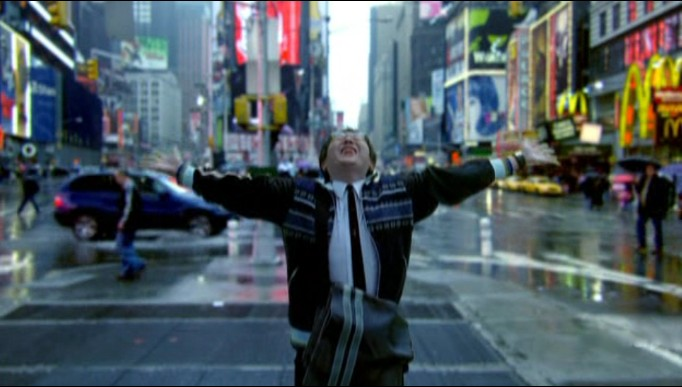
\includegraphics[scale=0.6]{Heroes_s01e02.jpg}
 	\caption{YATTAA!}
 	\label{fig-blog1}
\end{figure}

\YATTAA\ is \YATTAALong\ set. It contains classes for rapid development of simple data handling applications.

Sistema Genérico
\begin{itemize}
\item Menúes y landmarks               ->DONE
\item Módulos			               ->DONE
\item One template to rule them all    ->DONE
\item Abm -> Admin
\item Collection con orden y filtros
\item Impresión de reportes
\item Consultas estadísticas
\item Usuarios, permisos, login
\item ¿Context prediction?
\end{itemize}

\begin{verbatim}
Transform:

CozzuolModuleComponent -> ABCModule. El módulo tiene los menúes.

CozzuolComponent -> Workspace
CozzuolAdmin     -> ObjectAdmin


ActiveReference:: Medicina >> Problemas Médicos >> Problemas de "pepito 442/3" >> Nueva Consulta.

Menú landmark, menú navigacional, menú de operaciones, ActiveReference. Cuando llamo a una sub-funcionalidad, creo un menú que reemplaza al anterior, con una opción de 'volver', que vuelve al menú y al componente body anterior.

Un Workspace es un body, y un menú. Los elementos del menú, pueden llamar a otros Workspace. Un módulo tiene un nombre y un Workspace con body Inicial.

Otra opción es que el workspace entre a una de las opciones, pero que esta no tenga navegacion, sólo operaciones (¿Un Admin?).

Un Workspace común es el Admin. El Admin trabaja con multiple dispatching. Para un componente, presenta el Editor Default (PersistentObject), que trabaja con Reflection. Se puede modificar por uno específico hecho a mano.

El searcher es un Filterer, un Orderer y un List. Los 3 se obtienen con múltiple dispatching, y son Reflective por Default.

Permisos?

El módulo tiene un contexto (menúes). Cuando se llama a un componente, este carga sus menúes, y cuando se navega (hacia adelante o hacia atrás) descarga los menúes.

Está el ObjectsAdmin, que permite imprimir y crear un nuevo elemento (actions) y no tiene navigation. Cuando se hace click en un elemento, se llama a un NavigatedAdmin, con un ObjectAdmin adentro.

El ObjectAdmin registra sus menúes, y el ObjectsAdmin actúa en base a las acciones del ObjectAdmin. El NavigatedAdmin se registra en el ObjectAdmin, pero no usa los eventos. El NavigatedAdmin agrega la opción de 'volver', wrappeando al ObjectAdmin.

El ObjectAdmin es un Workspace? El NavigatedAdmin es un Workspace? Si agregamos ActiveReference, el NavigatedAdmin deja de ser importante (porque se puede volver desde ahí). Además, si agregamos que las colecciones se refresquen automáticamente, no es necesario hacer el 'callback refresh'.
\end{verbatim}

\end{document}